\chapter{Geschäftsvorfall}
\label{chap:vorfall}
Im Folgenden wird mit dem \gls{erp}-System ERPNext ein vorher festgelegter Geschäftsvorfall durchgeführt. \\
Um es so nah wie möglich an einem realen Unternehmen zu halten, wurde exemplarisch die fiktive \emph{Allgold Premium Molkerei GmbH} gewählt. Diese stellt im Allgäu bereits in dritter Generation hochwertige Molkereiprodukte her. Besonders bekannt ist sie für ihren wohlschmeckenden jungen Gouda.\\
Genau dieser soll auch im einem ausführlichen Geschäftsprozess hergestellt werden. Dafür haben wir uns für den gängigen Dreischritt \emph{Einkauf - Fertigung - Vertrieb} entschieden (\vgl Abbildung \ref{fig:geschVorfall}). Während der Durchführung werden auch an manchen Stellen Punkte angesprochen, die beim Experimentieren mit dem System besonders positiv oder negativ aufgefallen sind.
\begin{figure}[H]
  \centering
  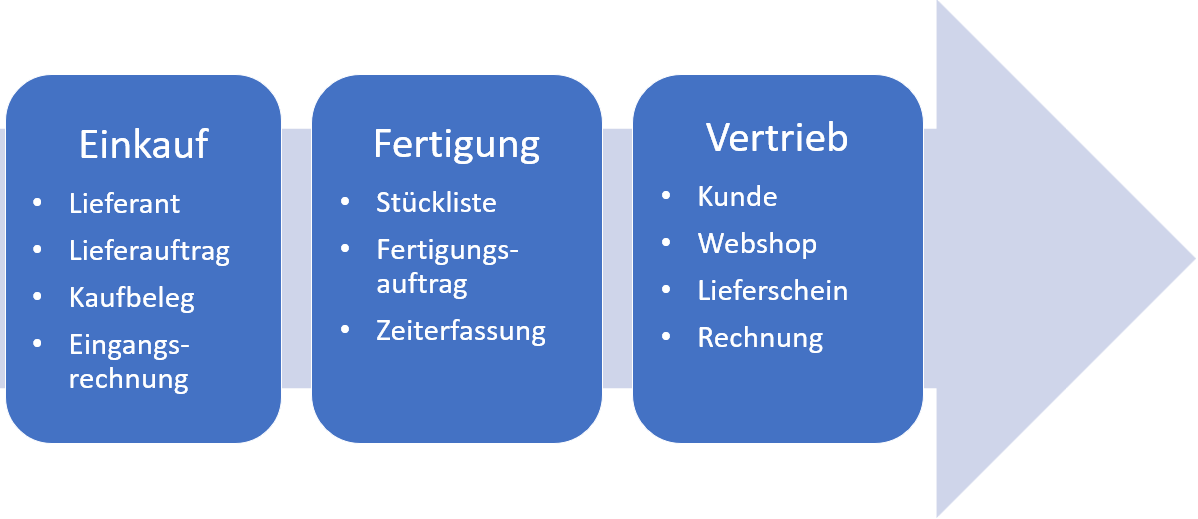
\includegraphics[width=\textwidth]{Bilder/Geschaeftsvorfall.PNG}
  \caption{Übersicht Geschäftsvorfall}
  \label{fig:geschVorfall}
\end{figure}
\emph{Hinweis:} Da die Vielzahl an Bildern zum Prozess den Rahmen dieser Seminararbeit sprengen würde, sind diese im Anhang zu finden. An den jeweiligen Stellen sind selbstverständlich diesbezüglich Verweise zu finden.

\section{Einkauf}
Da bei den einzelnen Abschnitten des Geschäftsprozesses nicht jeder kleinste Teil gezeigt werden kann, wurden bereits Vorkehrungen getroffen. So ist der Lieferant und die Rohprodukte Milch und Lab, sowie das Fertigprodukt Gouda bereits angelegt und mit entsprechenden Einkaufspreisen und Parametern versehen. Somit kann auf die anderen Prozessschritte und die Auffälligkeiten tiefer eingegangen werden.

\subsection{Lieferantenauftrag anlegen}
Zu Beginn dieses Prozesses muss für die Herstellung des Goudas Milch eingekauft werden. Mit einem neuen Lieferanten, Bauer Anton, haben wir uns im Vorfeld auf eine Lieferung von 2000 Litern Milch geeinigt. Da dieser Geschäftspartner bereits im System angelegt ist, kann mit diesem Datensatz eine Verknüpfung hergestellt werden (\vgl Abbildung \ref{fig:liefAuftrag}). Weil der Artikel Milch schon vorher angelegt worden ist, und hierbei ein Standardeinkaufspreis von 50 Cent eingetragen wurde, wird uns hier für 2000\ell\ Milch ein Gesamtbetrag von 1000€ vorgeschlagen. Natürlich kann an dieser Stelle der Stückpreis individuell abgeändert und die Summe vom System ausgerechnet werden. \\
Klickt man auf das kleine Dreieck ganz rechts des Artikels wird dem Benutzer eine Art Detailansicht angezeigt (\vgl Abbildung \ref{fig:auftrDetail}). Dort kann er noch einige Einstellungen tätigen, die sonst von den Standardeinstellungen ersetzt werden würden. \\
Nützlich ist allgemein auch, dass man stets einfach zu verknüpften Einträgen springen kann. Dazu muss lediglich der kleine Pfeil in jenem Eingabefeld gedrückt werden, in dem man sich gerade befindet (\vgl Abbildung \ref{fig:verlArtikel}).\\
Sieht man sich den Screenshot einmal genauer an, erkennt man an manchen Stellen schlechte oder nicht vorhandene Übersetzungen, wie beispielsweise bei\ \glqq Get last purchase rate\grqq. Diese Vorkommnisse häufen sich und decken sich mit dem, was die offizielle Übersetzungsseite preis gibt\footnote{Erreichbar unter: \url{https://translate.erpnext.com/}.}. Nur etwas mehr als die Hälfte der Strings der deutschen Übersetzung wurden verifiziert. Der andere Teil ist entweder maschinell übersetzt, oder wird in der Software noch im englischen Original angezeigt. \\
Wird der Auftrag nun abgeschlossen, muss der Lieferant natürlich auch über den Auftrag informiert werden. Dazu wird automatisch ein Popup-Fenster eingeblendet, sobald auf buchen gedrückt wird. Dort kann eine Email versendet werden, inklusive des Auftrags in PDF-Form (\vgl Abbildung \ref{fig:auftrPdf}). Dies erfordert die Einrichtung einer geeigneten Mail-Adresse in den Einstellungen, über die dann die Benachrichtigungen verschickt werden können.

\subsection{Ware empfangen}
Nach dem Absenden eines Lieferantenauftrages und der Bearbeitung seitens des Lieferanten kommt natürlich auch der Zeitpunkt, zu dem die Ware im Unternehmen eintrifft. Um eine Aktion im Rahmen des getätigten Lieferantenauftrags zu unternehmen, wählt man diesen einfach aus. Dort bekommt man dann direkt die häufigsten Aktionen vorgeschlagen (\vgl Abbildung \ref{fig:auftrUebersicht}). Oben links wird durch Ampelfarben und Text, wie hier \glqq Um zu empfangen und abzurechnen\grqq\ stets der aktuelle Stand des Lieferantenauftrags angezeigt. Das sieht man auch weiter unten beim Artikel Milch, der gelb gefärbt und somit noch nicht im Lager gebucht ist. \\
Um nun den Erhalt der Ware zu bestätigen und auf das vorher festgelegte, oder ein anderes Lager zu buchen muss auf das Plus-Zeichen neben Kaufbeleg gedrückt werden. Dadurch werden die bereits vorhandenen Informationen direkt in die nächste Maske übernommen (\vgl Abbildung \ref{fig:kaufbeleg}). Ein einfacher Klick auf den Text Kaufbeleg würde lediglich alle offenen Kaufbelege zu diesem Lieferantenauftrag anzeigen. \\
Sollte die angenommene Menge kleiner sein als die Bestellmenge, also nur eine Teillieferung erfolgt sein, kann das hierüber umgesetzt werden. Auch hier gilt wieder: Ein Klick auf das kleine Dreieck bietet dem Benutzer mehr Einstellungsmöglichkeiten. Nach dem Speichern des Kaufbelegs werden nicht ausgefüllte Felder, oder nicht erledigte Tätigkeiten von der Software hervorgehoben. Da die Molkerei stets die frische ihrer Produkte und einwandfreie Rohstoffe garantiert, wurde beim Rohmaterial Milch ein Flag für eine Qualitätskontrolle bei Eingang gesetzt. Deshalb fordert das System auf, diese durchzuführen (\vgl Abbildung \ref{fig:mittQual}). An dieser Stelle wird ein neuer Benutzer der Systems wahrscheinlich erst einmal etwas irritiert sein, da nicht sofort ersichtlich ist, durch welche Schaltfläche diese Kontrolle angestoßen werden kann. Dafür muss nämlich wieder in die Detailansicht des betreffenden Artikels gewechselt werden. Dort existiert dann im Abschnitt Lager und Referenz ein dementsprechender Punkt. Das System schlägt dem Benutzer an geeigneter Stelle stets schon vorhandene Elemente vor (soweit existent), oder lässt direkt ein neues anlegen, ohne dass der User aus der aktuellen Maske springen muss (\vgl Abbildung \ref{fig:auswQual}). \\
Die Qualitätskontrolle selbst (\vgl Abbildung \ref{fig:qualPruef}) ist schnell geschehen, da die Molkerei nur den Gehalt von Antibiotika in der Milch prüft. Danach lässt sich der Kaufbeleg ohne weitere Probleme buchen. \\
Geht man nun auf den Lieferantenauftrag zurück, fällt auf, dass sich der Status oben links auf \glqq Abrechnen\grqq\ geändert hat. Über das Plus bei Eingangsrechnung kann nun auch diese hinzugefügt werden. Im Lieferantenauftrag ist der Status danach auf \glqq Abgeschlossen\grqq\ gewechselt, aber die Lieferung ist noch unbezahlt. Der User könnte nun eine Zahlung über den Lieferantenauftrag anlegen, jedoch würde dabei der Bezug zur Rechnung verloren gehen. Geht man nun über die Verlinkung in die Eingangsrechnung des Auftrags und führt diese durch, wird ebendiese Verknüpfung vom System selbstständig hergestellt (\vgl Abbildung \ref{fig:zahlung}). Danach ändert sich der Status auf grün und \glqq Bezahlt\grqq. So bleibt die Zahlung auch später besser zuordenbar und Rechnungen bleiben nicht unabsichtlich unbezahlt.

\section{Fertigung}
Auch beim Bereich Fertigung wurden im Vorfeld bereits einige Dinge für die Stückliste angelegt. Dazu zählt der Arbeitsgang Lab hinzufügen (\vgl Abbildung \ref{fig:arbGang}) mit dem Arbeitsplatz Kessel (\vgl Abbildung \ref{fig:arbPlatz}).

\subsection{Stückliste anlegen}
Um den Gouda der \emph{Allgold Premium Molkerei GmbH} herzustellen wird eine Stückliste benötigt (\vgl Abbildung \ref{fig:stListe}). Diese kann neben benötigter Materialien auch Arbeitsgänge beinhalten. In diesem Beispiel verwenden wir zehn Liter Milch, sowie eine Einheit Lab. Dazu kommt ein Arbeitsgang, bei dem das Lab zu der Milch in den Kessel geschüttet wird. Aufgrund mangelnder Expertise unsererseits bei der Käseherstellung soll dies für den Moment schon genügen. \\
Bei dieser Stückliste wird automatisch ein Häkchen für den Standard gesetzt. Dies wird auch so belassen, damit die neue Stückliste später automatisch ausgewählt wird. 
Etwas unübersichtlich ist hierbei, dass die \glqq Operation Time\grqq\ für den Arbeitsgang in Minuten und nicht in Stunden angegeben werden muss. Dies sieht man erst, wenn man in die Detailansicht eines Arbeitsganges wechselt. Verwechselt man das bei unabsichtlich, werden die Betriebskosten vollkommen verfälscht. \\
ERPNext bietet zudem noch eine Möglichkeit, um eventuell anfallenden Ausschuss beziehungsweise Abfall bei der Herstellung zu berücksichtigen. Da dies aber bei diesem Beispiel nicht der Fall sein wird, kann das getrost übersprungen werden.

\subsection{Fertigungsauftrag erstellen}
Anhand der Stückliste kann nun ein Fertigungsauftrag für Gouda erstellt werden (\vgl Abbildung \ref{fig:fertAuftr}). Trägt man den zu fertigenden Artikel ein, wird automatisch die Standardstückliste zu diesem Artikel ausgewählt. Auch mehrstufige Stücklisten sind hierbei möglich, um diese Arbeit aber in einem überschaubaren Rahmen zu halten, wurde darauf verzichtet und auf eine normale Baukastenstückliste zurückgegriffen. \\
Beim Eintrag der herzustellenden Menge werden anhand der gewählten Stückliste die erforderliche Mengenanzahl der einzelnen Artikel, sowie die benötigte Zeit für die Arbeitsgänge ermittelt. Daraus ergeben sich dann für den Arbeitsgang auch die geplanten Betriebskosten.
An und für sich sind Pflichtfelder stets durch einen gelben Hintergrund gekennzeichnet. Beim Speichern und Buchen fällt dann jedoch auf, dass Hier auch Lager eingetragen werden müssen, welche diese Kennzeichnung davor nicht getragen haben. Das Eingangslager ist für die fertigen Erzeugnisse notwendig und das Fertigungslager dementsprechend für die Lagerung während der Fertigung. Danach lässt sich der Fertigungsautrag ohne Probleme ins System einbuchen un dessen Status wechselt auf \glqq Nicht begonnen\grqq\ (\vgl Abbildung \ref{fig:fertNichtBeg}). Im gleichen Augenblick wird ein dazugehöriges Timesheet erstellt.

\subsection{Zeiterfassung pflegen}
Nun müssen die Produktion gestartet und die entsprechenden Materialien aus dem Lager transferiert werden (\vgl Abbildung \ref{fig:matTransfer}). Dabei könnte auch nur eine Teilmenge hergestellt werden, was wir in diesem Beispiel jedoch nicht tun werden. Alle benötigten \glqq Einzelteile\grqq\ sind verfügbar und können somit verschoben werden (\vgl Abbildung \ref{fig:lagBuchung}). Nach Beendigung des Fertigungsauftrages mit dem von uns erdachten Arbeitsschritts kann die benötigte Zeit ins System eingebucht werden (\vgl Abbildung \ref{fig:timeSheet}). Dabei wird zuerst die veranschlagte Zeit voreingetragen. Sollte der Mitarbeiter mehr oder weniger Zeit benötigt haben, könnte er das an dieser Stelle eintragen. Das hätte dann wiederum Einfluss auf die Kosten des Arbeitsganges und somit des Herstellungspreises unseres Goudas. \\
Ist unser Gouda gefertigt, muss eine neue Lagerbuchung angestoßen werden, um die Roh-Artikel aus dem Lager zu nehmen und den Gouda ins Lager der Fertigerzeugnisse zu legen (\vgl Abbildung \ref{fig:beenFertig}).
TODO: - In Realität anderer Mitarbeiter
- Auswertung der Zeiten?
- Lohnanzeige?
- Mehrarbeit?

\section{Vertrieb}
Für den Vertrieb des Goudas  hat ERPNext nicht nur die Möglichkeit Kunden über das \gls{erp}-System durch einen Mitarbeiter der Molkerei anzulegen, sondern auch den Bestellprozess direkt durch den Kunden über einen Webshop anzustoßen. Dadurch wird das System direkt zur Verkaufsplattform.\\
In diesem Beispiel will ein der Kunde \glqq Großhandel Gummersbach\grqq\ Gouda für sein Geschäft einkaufen.

\subsection{Kunden anlegen}
Der Kunde kann sich unter dem Reiter \glqq Anmelden\grqq\ der Webseite einen neuen Account anlegen. Dazu muss er seinen vollständigen Namen (bzw. den Namen des Geschäfts), sowie eine Email-Adresse angeben (\vgl Abbildung \ref{fig:regKunde}). Dadurch kommt er nie mit der Verwaltungsplattform, wie sie ein Mitarbeiter benutzt, in Berührung. Nach erfolgreicher Registrierung wird dem Kunden eine Email zugeschickt (\vgl Abbildung \ref{fig:regMail}).

\subsection{Verkaufsauftrag erstellen}

\subsection{Zahlung tätigen}
- eig. Payment-Gateway, dazu auch passende Einstellung im System vorhanden...

\subsection{Ware ausliefern}

\section{Fazit}
- angenehm zu benutzendes ERP-System, anfangs etwas bunt, aber auf Corporate Design anpassbar
- Customizings auf Clientseite einfach zu tätigen
- man kann direkt in verknüpfte Bereiche durch Pfeilchen springen

- Während Anlegen Fertigungsauftrag Systemabsturz (Screenshot!) - Wo liegt der Fehler? Ausgabe von ERPNext
- Zuordungen Produkt <-> Lieferant fehlen
- an manchen Stellen ist die Benutzerführung nicht durchgängig (Stichwort Plus-Zeichen oder Make?)
- die Übersetzung bereitet manchmal Schwierigkeiten
- nicht von vorneherein auf den deutschen Sprachraum eingestellt (Stichwort Datumssystem, Geldsystem (Punkte, Kommas), komische Rundungsregeln???)
- Man hat nicht verschiedene Reiter, sondern muss über die zurück-Funktion des Browsers navigieren; oder das Hauptmenü
